\documentclass[a4paper]{article}
\usepackage[francais]{babel}
\usepackage{graphicx}
\usepackage{wrapfig}
\usepackage[utf8]{inputenc}
\usepackage{soul}
\usepackage{scrpage2}
\usepackage{titlesec}
\usepackage{multicol}
\usepackage{tikz}
\usepackage{hyperref}
\usepackage{pbox}
\usepackage{hyperref}
\usepackage[margin=1.5cm]{geometry}
\usepackage{amsthm}
%\usepackage{multicolumn}
\usepackage{tabularx}
\usepackage[scaled]{helvet}
\usepackage{listings}
\usepackage{appendix}
\usepackage{float}

\newcommand{\comment}[1]{}

\definecolor{javared}{rgb}{0.6,0,0} % for strings
\definecolor{javagreen}{rgb}{0.25,0.5,0.35} % comments
\definecolor{javapurple}{rgb}{0.5,0,0.35} % keywords
\definecolor{javadocblue}{rgb}{0.25,0.35,0.75} % javadoc

\lstset{language=Java,
basicstyle=\ttfamily,
keywordstyle=\color{javapurple}\bfseries,
stringstyle=\color{javared},
commentstyle=\color{javagreen},
morecomment=[s][\color{javadocblue}]{/**}{*/},
numbers=left,
numberstyle=\tiny\color{black},
%stepnumber=2,
numbersep=10pt,
tabsize=4,
showspaces=false,
showstringspaces=false}

\title{Rapport projet ARA 2017-2018}
\author{Mickael Rudek, Oskar Viljasaar}

\begin{document}
\maketitle


\tableofcontents
\pagebreak
\section{Exercice 1 - Implémentation d'un MANET dans PeerSim}
\subsection{Algorithme de déplacement d'un noeud (Question 1)}

\begin{verbatim}
Movement protocol:
- if not moving
    - assign random speed lower than max
- moving
    - use `PositioningStrategiesFactory` to get next destination
    - Calc distance to next destination
    - if too far to reach `destination` in one hop
        - calculate next `x` and `y`
        - move to that position
    - if destination reached, stop
    - else continue running
\end{verbatim}
L'algorithme utilise le protocole de déplacement suivant:
Une valeur de la vitesse est aléatoirement choisie dans l'intervalle
$ \left[ \texttt{speed\_min}; \texttt{speed\_max} \right] $.
Vu qu'on est en temps discretisé, $distance\_to\_next$ représente la
distance parcourue en une unité de temps.
Une fois la destination atteinte, le noeud s'arrête pendant un tic,
 sinon il boucle en demandeant une nouvelle destination de la
 stratégie de déplacement.


 \subsection{Contenu du fichier de configuration pour la question 2}

\begin{verbatim}
simulation.endtime 50000
random.seed 5
network.size 10
init.initialisation Initialisation
control.graph GraphicalMonitor
control.graph.positionprotocol position
control.graph.time_slow 0.0002
control.graph.step 1
\end{verbatim}

\subsection{Questions 3 et 4}
Voir la sous-section 1.6.

\subsection{Implémentation de l'interface \texttt{Emitter} (Question 5)}

\subsection{Influence des stratégies sur la connexité du graphe (Questions 3, 4, 8)}
\begin{minipage}{0.45\textwidth}

%\begin{itemize}

  \textsl{Strategy1InitNext} donne des positions initiales et destinations
aléatoires dans le terrain pour chaque noeud.

\textsl{Strategy3InitNext} donne des positions initiales et
    destinations vers le milieu du terrain, dans un rayon de $ \texttt{scope} -
\texttt{marge} $, assurant un graphe
    connexe.

    \textsl{Strategy2Next} rend les noeuds immobiles, la connexité du
      graphe dépend du placement initial des noeuds.

     \textsl{Strategy4Next} assume que le graphe est connexe à
    l'initiation. Elle va déplacer un nœud dans le graphe en
    s'assurant qu'à la fin, le graphe soit toujours connexe. La
    connexité du graphe dépend du placement initial des noeuds.

    \textsl{Strategy5Init} place les noeuds en haut à droite du terrain,
      chaque noeud est placé dans le scope d'un autre noeud.
      Le graphe est initialement connexe.

      \textsl{Strategy6Init} place les noeuds en étoile au milieu du
        terrain, le graphe est donc initialement connexe.\\

\end{minipage}%
\hfill
\begin{minipage}{0.5\textwidth}
    \begin{table}[H]
\centering
    \begin{tabular}{| l | l | l |}
  \hline
  \textsl{SPI} & \textsl{SD} & \textbf{Connexe}\\
  \hline
  Strategy1InitNext & Strategy1InitNext & non\\
  \hline
  Strategy1InitNext & Strategy2Next &  non\\
  \hline
  Strategy1InitNext & \textbf{Strategy3InitNext} & \textbf{oui}\\
  \hline
  Strategy1InitNext & Strategy4Next & non \\
  \hline
  Strategy3InitNext & Strategy1InitNext & non \\
  \hline
  \textbf{Strategy3InitNext} & Strategy2Next & \textbf{oui} \\
  \hline
  Strategy3InitNext & \textbf{Strategy3InitNext} & \textbf{oui}\\
  \hline
  \textbf{Strategy3InitNext} & Strategy4Next & \textbf{oui}\\
  \hline
  Strategy5Init & Strategy1InitNext & non \\
  \hline
  \textbf{Strategy5Init} & Strategy2Next & \textbf{oui}\\
  \hline
  Strategy5Init & \textbf{Strategy3InitNext} & \textbf{oui} \\
  \hline
  \textbf{Strategy5Init} & Strategy4Next & \textbf{oui} \\
  \hline
  Strategy6Init & Strategy1InitNext & non\\
  \hline
  \textbf{Strategy6Init} & Strategy2Next & \textbf{oui} \\
  \hline
  Strategy6Init & \textbf{Strategy3InitNext} & \textbf{oui}\\
  \hline
  \textbf{Strategy6Init} & Strategy4Next & \textbf{oui}\\
  \hline
\end{tabular}
    \caption{Impact des différentes SPI et SD sur la connexité du graphe}
    \label{table:SPISDGraphe}
  \end{table}
\end{minipage}
%Différentes combinaisons de ces stratégies et la connexité du graphe
%en résultant sont résumés dans la table \ref{table:SPISDGraphe}.


\subsection{Impact de la portée sur la densité du graphe (Questions 10 et 11)}

\begin{minipage}{0.40\textwidth}
Dans la stratégie 1, l'étendue de la portée a un impact sur la
connexité du graphe, la stratégie de déplacement étant celle de
choisir des destinations aléatoires dans le terrain. Il est plus
facile donc de faire un graphe connexe en prenant une valeur assez
grande pour la portée.

La stratégie 3 donnant un graphe connexe dès
le début, les noeuds disposent déjà d'un nombre de voisins important.
Augmenter la portée pour la stratégie 3 a tendance à légèrement faire
diminuer la densité du graphe. Cela peut être expliqué par la distance
aléatoire pour la prochaine destination, tirée entre
\texttt{NextDestinationStrategy.minimum\_distance} et $scope - marge$, sachant
que $marge$ est plutôt petit (20) et reste constant, alors que la
portée peut varier jusqu'à 1000. Le graphe, dans la stratégie 3, est beaucoup
plus étendu, et les noeuds peuvent avoir moins d'arcs directs
entre eux.

\end{minipage}%
\hfill
\begin{minipage}{0.55\textwidth}
  \begin{table}[H]
    \centering
    \begin{tabular}{|c|c|c|c|c|c|}
      \hline
Portee & SPI & SD & D & E/D & ED/D \\
      \hline
125 & 1 & 1 &  1.00 +- 0.02& 0.27 +- 0.02 & 0.04 +- 0.00 \\
250 & 1 & 1 &  3.81 +- 0.10& 0.14 +- 0.00 & 0.04 +- 0.00 \\
375 & 1 & 1 &  8.02 +- 0.20& 0.13 +- 0.02 & 0.09 +- 0.02 \\
500 & 1 & 1 & 12.83 +- 0.06& 0.11 +- 0.02 & 0.09 +- 0.02 \\
625 & 1 & 1 & 18.77 +- 0.54& 0.11 +- 0.00 & 0.13 +- 0.01 \\
750 & 1 & 1 & 24.49 +- 0.13& 0.10 +- 0.00 & 0.16 +- 0.02 \\
875 & 1 & 1 & 29.92 +- 0.47& 0.09 +- 0.00 & 0.16 +- 0.02 \\
1000& 1 & 1 & 35.66 +- 0.44& 0.07 +- 0.01 & 0.11 +- 0.04 \\
\hline
125 & 3 & 3 & 29.94 +- 0.25 & 0.09 +- 0.00 & 0.17 +- 0.02 \\
250 & 3 & 3 & 26.78 +- 0.27 & 0.10 +- 0.01 & 0.21 +- 0.05 \\
375 & 3 & 3 & 25.82 +- 0.41 & 0.09 +- 0.00 & 0.16 +- 0.01 \\
500 & 3 & 3 & 25.75 +- 0.58 & 0.10 +- 0.00 & 0.15 +- 0.02 \\
625 & 3 & 3 & 25.52 +- 0.33 & 0.09 +- 0.00 & 0.15 +- 0.03 \\
750 & 3 & 3 & 25.80 +- 0.23 & 0.10 +- 0.00 & 0.16 +- 0.02 \\
875 & 3 & 3 & 25.61 +- 0.47 & 0.10 +- 0.00 & 0.16 +- 0.02 \\
1000& 3 & 3 & 25.21 +- 0.31 & 0.10 +- 0.00 & 0.16 +- 0.02 \\
\hline
    \end{tabular}
\caption{Valeurs obtenues pour la question 10, normalisées sur 100 itérations}
\end{table}
\end{minipage}
\vfill

\begin{figure}[H]
  \centering
  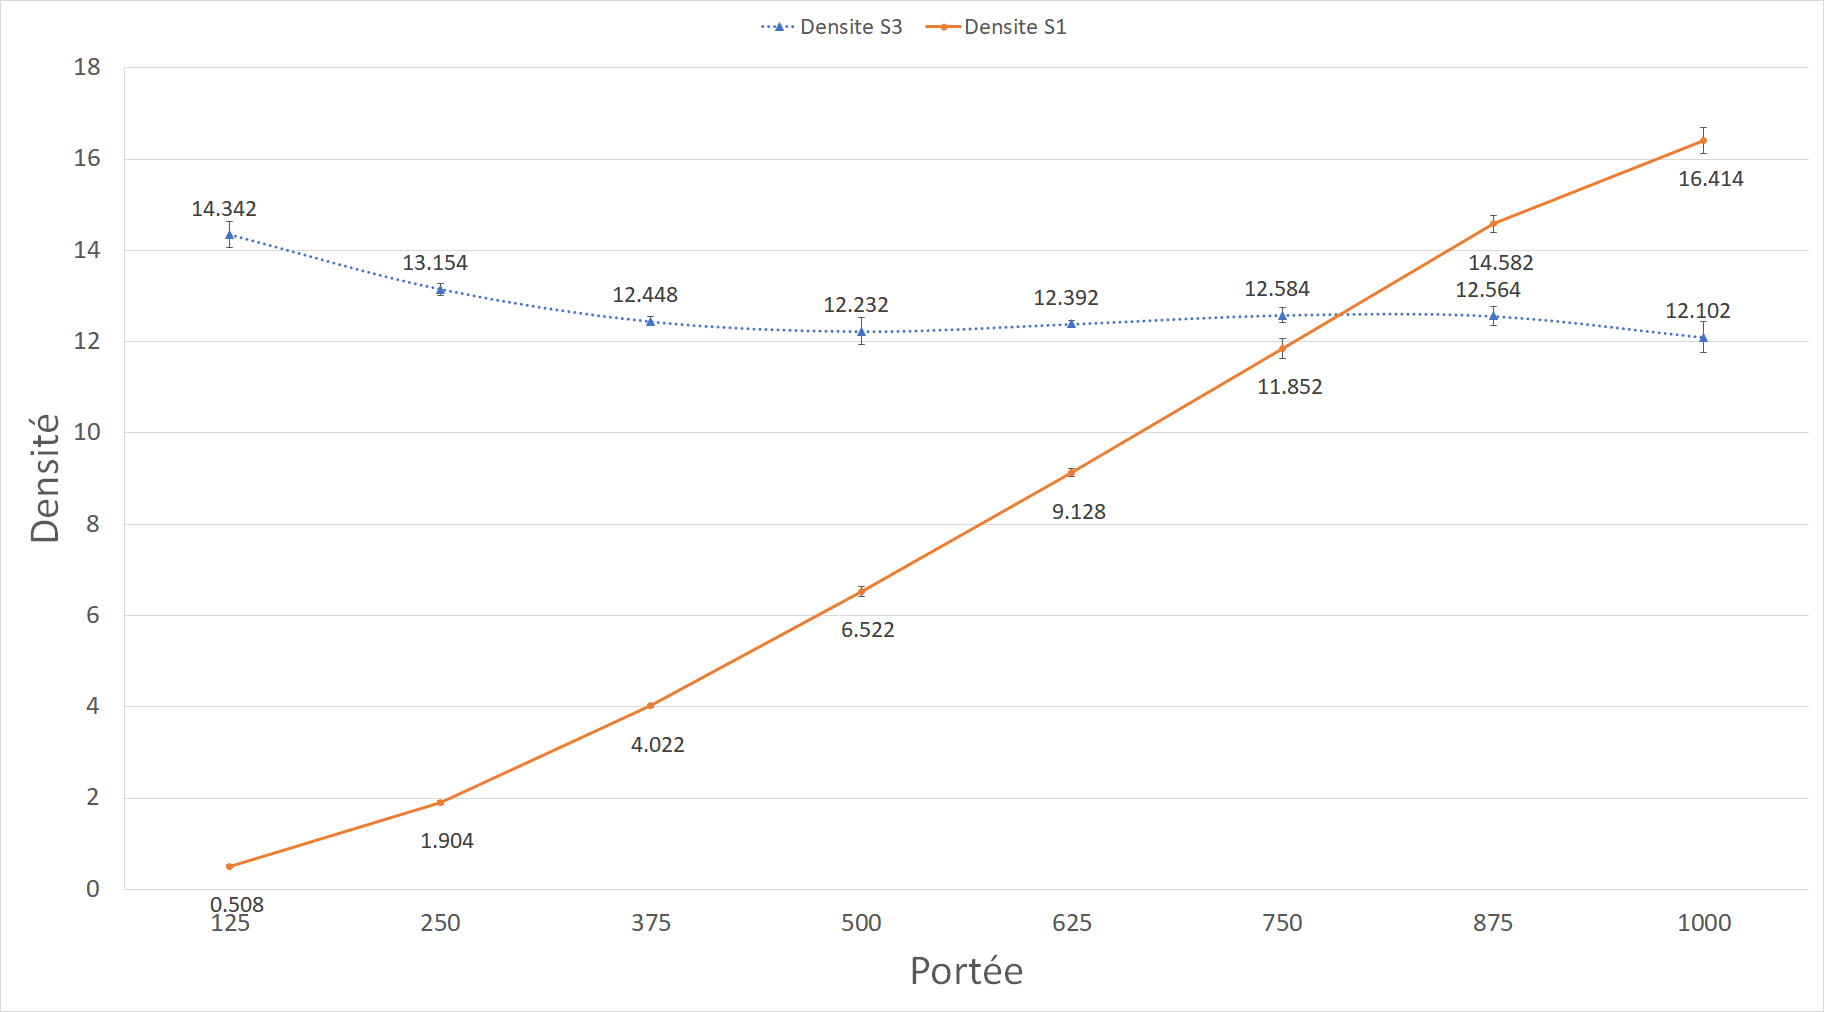
\includegraphics[width=\textwidth]{images/q10-11-s1and2.png}
  \caption{Impact de la portée sur la densité avec la stratégie 1 (orange) et la 3 (bleu).}
  \label{fig:S1-S3-portee}
\end{figure}


\section{Exercice 2 - Étude de protocoles de diffusion}
\subsection{Impact du nombre de noeuds sur la densité du
  graphe (Question 1)}
\begin{minipage}{0.6\textwidth}
  Selon le graphe, le réseau est plutôt chaotique sur un nombre de
  noeuds faible, allant jusqu'à 50 selon nos résultats. L'écart-type
  entre les différentes valeurs mesurées est fort, le réseau peut
  avoir du mal à s'interconnecter selon les différentes valeurs
  initiales aléatoires prises. À partir de 50 noeuds, le réseau a un
  comportement attendu et la densité croît de manière relativement
  stable, avec un écart-type faible entre les mesures.

  En dessous de 50 noeuds, on ne peut donc pas forcément s'attendre à
  un placement de noeuds idéal, de manière à ce que tous les noeuds
  soient connectés avec beaucoup de voisins à proximité.
  \vfill
\end{minipage}%
\hfill
\begin{minipage}{0.35\textwidth}
\begin{tabular}{p{\textwidth} l}
\begin{table}[H]
  \centering
  \begin{tabular}{|l|r|r|}
    \hline
    Taille & D-end & ED/D end \\ \hline
    10  &  3.32 +- 0.00 & 0.26 +- 0.00 \\ \hline
     20  &  6.88 +- 1.03 & 0.55 +- 0.30 \\ \hline
     30  & 10.92 +- 2.11 & 0.28 +- 0.20 \\ \hline
     40  & 16.04 +- 4.00 & 0.17 +- 0.11 \\ \hline
     50  & 21.95 +- 4.95 & 0.08 +- 0.01 \\ \hline
     60  & 23.37 +- 6.02 & 0.13 +- 0.05 \\ \hline
     70  & 23.11 +- 4.74 & 0.08 +- 0.03 \\ \hline
     80  & 27.26 +- 1.76 & 0.07 +- 0.03 \\ \hline
     90  & 37.59 +- 3.83 & 0.06 +- 0.02 \\ \hline
     100 & 35.38 +- 3.23 & 0.04 +- 0.01 \\ \hline
     120 & 37.78 +- 5.27 & 0.03 +- 0.01 \\ \hline
     140 & 47.42 +- 12.2 & 0.04 +- 0.01 \\ \hline
     160 & 49.15 +- 10.2 & 0.03 +- 0.02 \\ \hline
     180 & 62.37 +- 5.31 & 0.03 +- 0.01 \\ \hline
     200 & 50.33 +- 7.25 & 0.02 +- 0.01 \\ \hline
  \end{tabular}
  \caption{Valeurs obtenues pour la question 1, normalisés sur 100 itérations}
\end{table}
\end{tabular}
\end{minipage}


\begin{figure}[H]
\begin{minipage}{\textwidth}
  \centering
    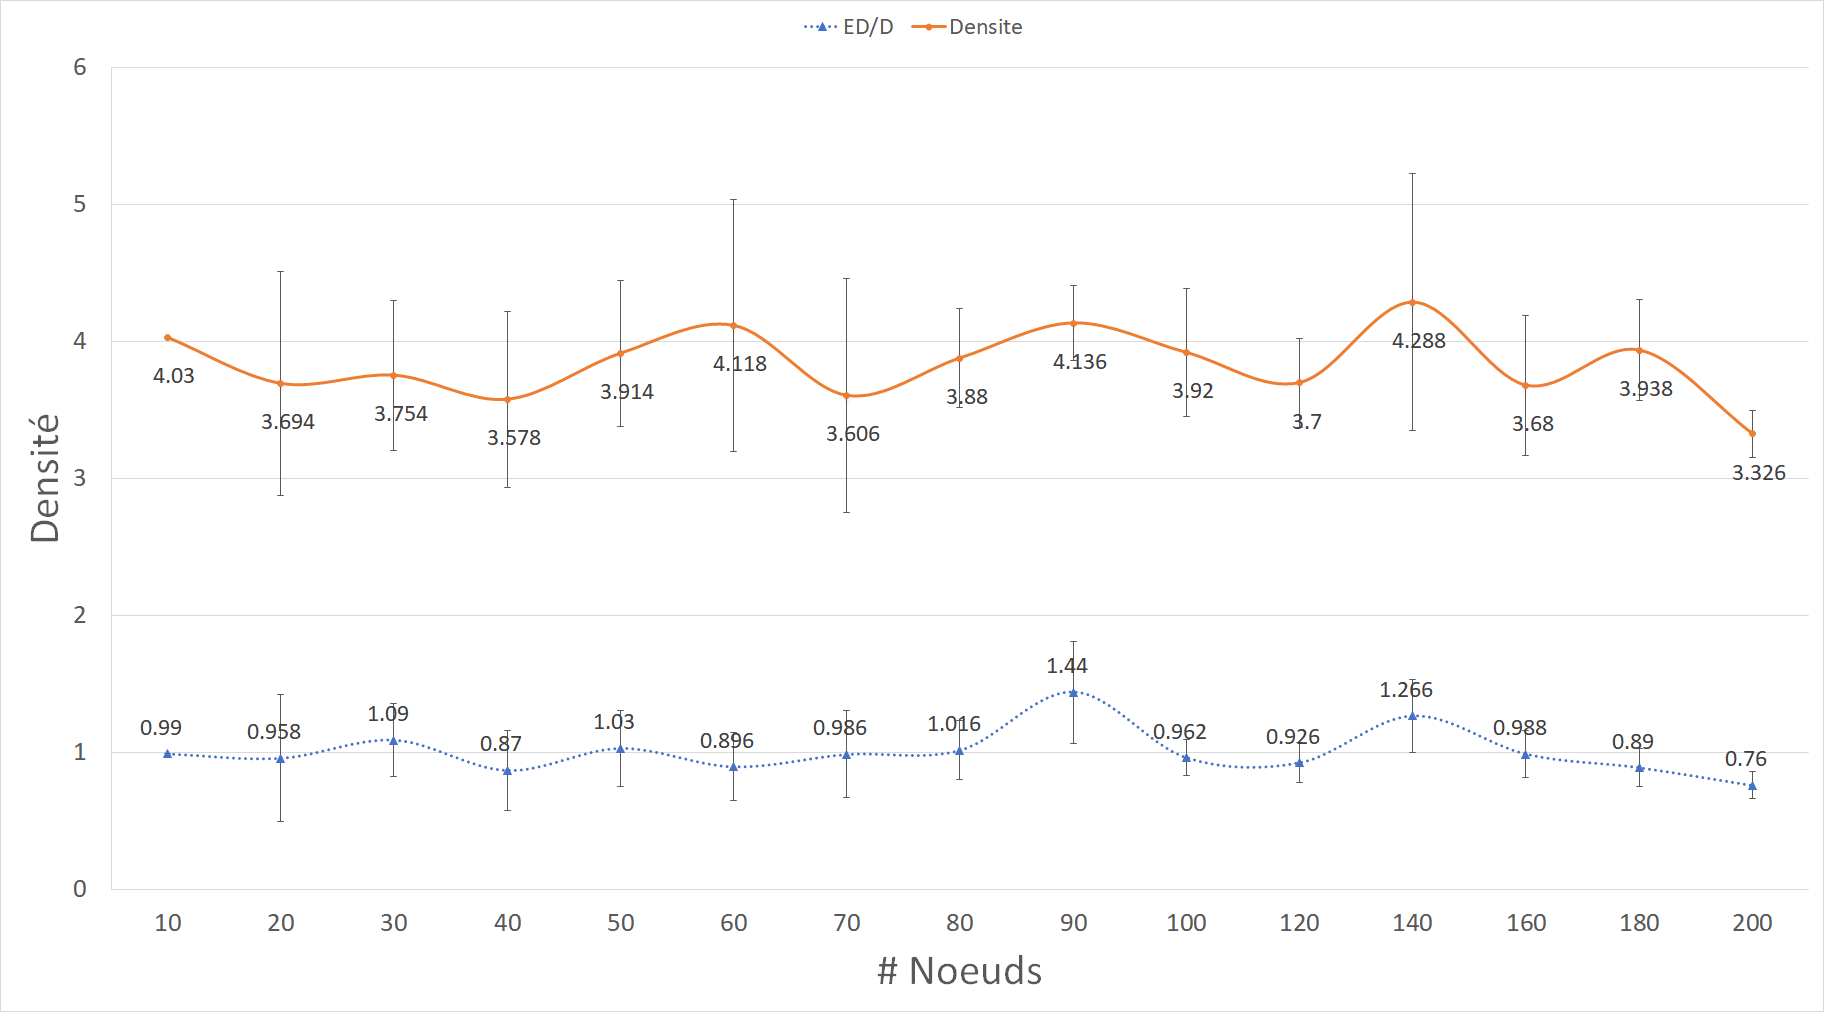
\includegraphics[width=\textwidth]{images/ex2.png}
    \caption{Impact du nombre de noeuds sur la densité et sa variation possible
      pendant une simulation, avec les stratégies $SPI5$ et $SD4$.}
\end{minipage}
\end{figure}

\subsection{Question 2 (\texttt{EmitterCounter})}
On a défini une classe abstraite \texttt{EmitterCounter} utilisant le
design pattern \textsl{Strategy}, en rendant la méthode \texttt{emit}
abstraite. Une sous-classe concrète de celle-ci implémente une politique particulière d'émission
(\texttt{FloodingEmitter}, \texttt{ProbabilisticEmitter}, ...) et rend
le nombre de messages envoyés selon cette politique.
Cette information est destinée à \texttt{GossipProtocol} qui se charge
de la délivrance (ou non) du message selon si le noeud émetteur se
trouve encore dans la portée du récepteur.

On a essayé d'implémenter
cette politique de délivrance au niveau de l'émetteur
(\texttt{EmitterCounter}) en le faisant traiter des réceptions de
messages de son protocole encapsulant des messages de n'importe quel
protocole au-dessus de lui-même, mais le simulateur rendait trop difficile de détecter
une terminaison de manière simple. La fonction EDSimulator.add(0, ..)
rajoute un évènement à la fin de la file d'éxecution, mais on voulait
faire un traitement juste après la délivrance du message par \texttt{EmitterCounter}.

\subsection{Question 4 (\texttt{FloodingEmitter})}

\subsection{Question 5 (\texttt{ProbabilisticEmitter})}

Le pourcentage de messages reçus augmente clairement selon la
probabilité. Selon les résultats expérimentaux, il faut définir une probabilité autour
de 0.3 afin d'obtenir une atteignabilité d'au moins 90\%. À partir
d'une densité de graphe de 5, l'atteignabilité ne descend pas
en-dessous des 80\%. Pour obtenir une atteignabilité moyenne du graphe
d'au moins 99\%, il faudrait utiliser une probabilité d'au moins 0.7.

Les courbes figurant sur le graphe représentent les différentes
classes d'atteignabilité définies dans la question de l'exercice. La
courbe grise et orange montrent qu'il est vite possible d'atteindre la
majorité du graphe, même avec une densité faible.

\begin{figure}[H]
\begin{minipage}{\textwidth}
  \centering
    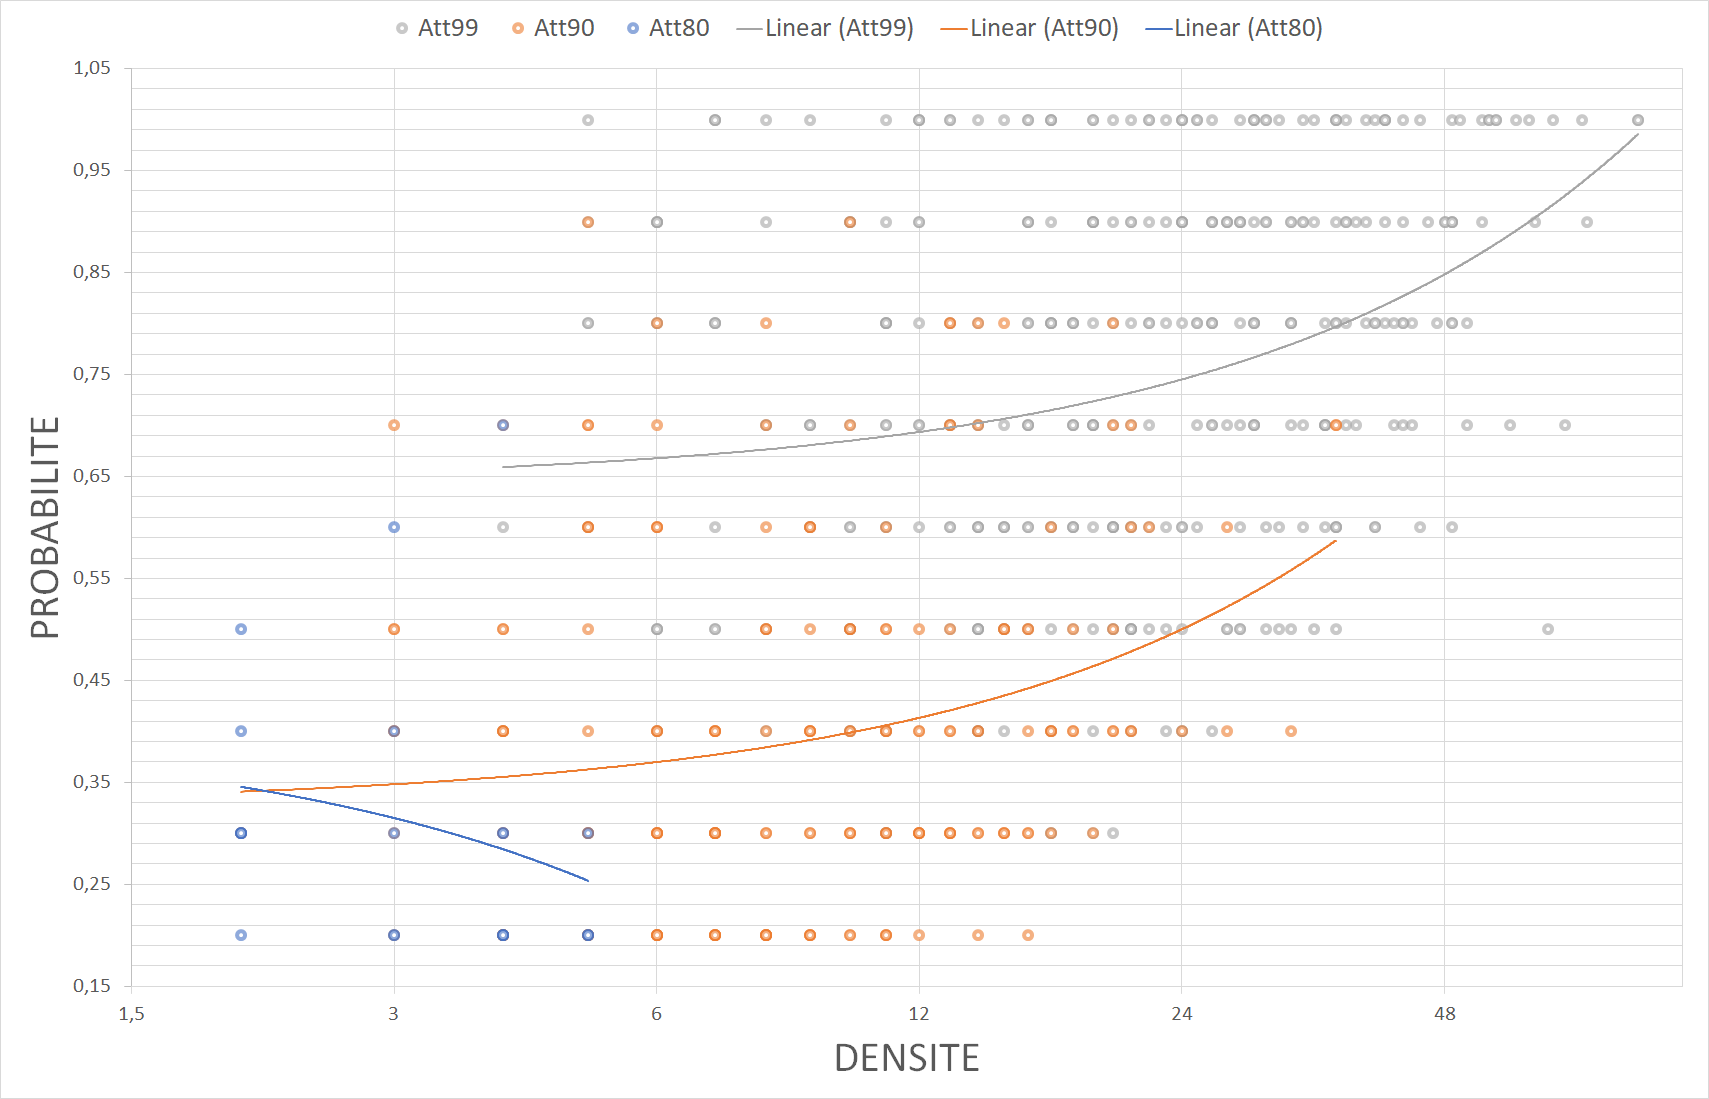
\includegraphics[width=\textwidth]{images/ex2q5-log-trendlines.png}
    \caption{Probabilité en fonction de la densité. Le graphe contient
    les valeurs de 5 éxecutions différentes pour un même ensemble de
    valeurs initiales (nombre de noeuds/densité et probabilité).}
\end{minipage}
\end{figure}

\subsection{Question 6 (\texttt{InverseProportionalEmitter})}

\subsection{Question 7 (\texttt{DistanceEmitter})}


\pagebreak


\begin{appendix}
  \section{Compilation, lancement du code et jeux de test}
  \subsection{\texttt{src/Makefile}}
    Un fichier \texttt{Makefile} est inclus dans le dossier
    \texttt{src}. Celui-ci reconnaît les directives:
    \begin{itemize}
    \item \texttt{make} compile le projet.
    \item \texttt{make run} lance une instance de simulation telle que
      spécifiée dans \texttt{src/manet/cfg\_initial.txt}.
    \item \texttt{make clean} nettoie le projet des compilés.
    \item \texttt{make bench\_clean} nettoie le dossier \texttt{src}
      des dossiers de résultats des benchmarks.\\
    \end{itemize}

    Le \texttt{Makefile} admet par ailleurs deux variables:
    \begin{itemize}
    \item \texttt{DIR\_PEERSIM=<chemin>}: le dossier d'installation de
      Peersim, qu'il faudra \textbf{obligatoirement} soit modifier,
      soit spécifier dans \texttt{make} et \texttt{make run}.
    \item \texttt{CFG=<chemin>}: le chemin d'un fichier de
      configuration Peersim, initialisé à \texttt{src/manet/cfg\_initial.txt} par défaut.
    \end{itemize}

    \subsection{\texttt{src/bench.pl}}
    Exemple: \texttt{./bench.pl <chemin\_peersim>}

    Le script crée un dossier \texttt{resultats/bench\_<date>} où seront stockés les
    résultats pour la question 8 de l'exercise 1. Le dossier contiendra
    les fichiers de configuration pour les expériences sous le nom
    \texttt{cfg\_bench\_<scope>\_<SPI>\_<SD>}, les résultats d'autres
    fichiers, de même nom avec l'extension \texttt{.result}. Ces derniers contiennent les résultats de 100 expériences avec autant de différentes graines aléatoires.

    \subsection{\texttt{src/bench.py}}
    exemple: \texttt{bench.py <chemin\_results>}

    Dans le dossier \texttt{<chemin\_results>} doivent se trouver les fichiers résultats créés par \texttt{bench.pl}. Utilisé pour les resultats de benchmark, pour remplir les tableaux.

Exemple de sortie:
\begin{verbatim}
/ara/src/results/cfg_bench_500_3_3.result
| 2.3830 +- 0.0684 | 0.4320 +- 0.0426 | 0.2300 +- 0.0335 |

/ara/src/results/cfg_bench_875_3_3.result
| 2.3390 +- 0.1023 | 0.4400 +- 0.0369 | 0.2140 +- 0.0201 |

/ara/src/results/cfg_bench_750_1_1.result
| 2.2740 +- 0.1165 | 0.4630 +- 0.0518 | 0.2320 +- 0.0325 |

/ara/src/results/cfg_bench_375_1_1.result
| 0.7130 +- 0.0447 | 0.6550 +- 0.0457 | 0.1790 +- 0.0230 |
\end{verbatim}
Les valeurs correspondent à des moyennes avec écarts-type, obtenus sur
100 itérations sur chaque combinaison de SPI et SD.



\subsection{\texttt{src/bench\_ex2.py}}
exemple: \texttt{bench\_ex2.py <chemin\_results>}
Ce script traite les resultats des simulations de l'exercise deux. Il prepare deux fichiers, stockes dans le dossier specifie dans l'appel - \texttt{summary.csv} et \texttt{summary\_all.csv}.

\texttt{summary.csv} contient des valeurs normalises sur le nombre d'experiences, tandis que \texttt{summary\_all.csv} store simplement tout les resultats, sans compter les moyennes.


\subsection{\texttt{bench-ex2q\{1,3,4\}.pl}}
Exemple: \texttt{./bench-ex2q\{1,3,4\}.pl <chemin\_peersim>}

Le script crée un dossier \texttt{resultats/bench\_<date>\_ex2q\{1,3,4\}} où
seront stockés les résultats des différentes exécutions, les noms des fichiers
étant différentiés par la taille du réseau.

\subsection{\texttt{bench-ex2q5.pl}}
Exemple: \texttt{./bench-ex2q5.pl <chemin\_peersim>}
Le script crée un dossier \texttt{resultats/bench\_<date>\_ex2q5} où
seront stockés les résultats des différentes exécutions, les noms des
fichiers étant différentiés par la taille du réseau, la probabilité
donnée et le numéro de l'itération.

Les scripts de l'exercice 2 (hormis la question 1) sortent un fichier
par exécutions, de forme:
\begin{verbatim}
Att;Ed-Att;ER;Ed-ER
D;ED;ED/D
\end{verbatim}


\section{Extraits de code}
\subsection{Implémentation de l'interface \texttt{Emitter} (Exercice 1
  Question 5)}
\begin{lstlisting}
package manet.communication;

import manet.Message;
import manet.positioning.Position;
import manet.positioning.PositionProtocol;
import peersim.config.Configuration;
import peersim.core.Network;
import peersim.core.Node;
import peersim.core.Protocol;
import peersim.edsim.EDSimulator;

public class EmitterImpl implements Emitter {

    private int latency;
    private int scope;
    private int this_pid;
    private int position_protocol;

    private static final String PAR_LATENCY = "latency";
    private static final String PAR_SCOPE = "scope";
    private static final String PAR_POSITIONPROTOCOL = "positionprotocol";

    public EmitterImpl(String prefix) {
        String tmp[]=prefix.split("\\.");
        this_pid=Configuration.lookupPid(tmp[tmp.length-1]);
        this.position_protocol=Configuration.getPid(prefix+"."+PAR_POSITIONPROTOCOL);
        this.latency = Configuration.getInt(prefix + "." + PAR_LATENCY);
        this.scope = Configuration.getInt(prefix + "." + PAR_SCOPE);
    }

    @Override
    public void emit(Node host, Message msg) {
        PositionProtocol prot =
            (PositionProtocol) host.getProtocol(position_protocol);

        for (int i=0; i < Network.size(); i++) {
            Node n = Network.get(i);
            PositionProtocol prot2 =
                (PositionProtocol) n.getProtocol(position_protocol);
            double dist =
                prot.getCurrentPosition().distance(prot2.getCurrentPosition());
            if (dist < scope && n.getID() != host.getID()) {
                EDSimulator.add(latency, new Message(msg.getIdSrc(),
                                                     n.getID(),
                                                     msg.getTag(),
                                                     msg.getContent(),
                                                     msg.getPid()),
                                                     n, msg.getPid());
            }
        }

    }

    @Override
    public int getLatency() { return latency; }

    @Override
    public int getScope() { return scope; }

    @Override
    public Object clone(){
        EmitterImpl res=null;
        try {
            res=(EmitterImpl)super.clone();
        } catch (CloneNotSupportedException e) {}
        return res;
    }
}
\end{lstlisting}

\subsection{Implémentation de l'interface \texttt{NeighborProtocol}
  (Exercice 1 Question 6)}


\begin{lstlisting}
package manet.detection;

import manet.Message;
import manet.communication.EmitterImpl;
import peersim.config.Configuration;
import peersim.core.Node;
import peersim.edsim.EDProtocol;
import peersim.edsim.EDSimulator;

import java.util.ArrayList;
import java.util.List;

public class NeighborProtocolImpl implements NeighborProtocol, EDProtocol {
    private int this_pid;
    private int period;
    private int timer_delay;
    private int listener_pid;

    private static final String PAR_PERIOD = "period";
    private static final String PAR_TIMERDELAY = "timer_delay";
    private static final String PAR_LISTENER_PID = "listenerpid";
    Integer timeStamp = 0;

    private List<Long> neighbor_list;

    public NeighborProtocolImpl(String prefix) {
        neighbor_list = new ArrayList<>();

        String tmp[]=prefix.split("\\.");
        this_pid= Configuration.lookupPid(tmp[tmp.length-1]);
        this.period = Configuration.getInt(prefix+"."+PAR_PERIOD);
        this.timer_delay = Configuration.getInt(prefix + "." + PAR_TIMERDELAY);
        this.listener_pid = Configuration.getPid(prefix + "." + PAR_LISTENER_PID,-1);
        }

    @Override
    public List<Long> getNeighbors() { return neighbor_list; }

    @Override
    public Object clone() {
        NeighborProtocolImpl res = null;
        try {
            res = (NeighborProtocolImpl) super.clone();
            neighbor_list = new ArrayList<>();
            timeStamp = new Integer(0);
        } catch (CloneNotSupportedException e) {

        }
        return res;
    }

    @Override
    public void processEvent(Node node, int pid, Object event) {
        int emitter_pid = Configuration.lookupPid("emitter");
        EmitterImpl impl = (EmitterImpl) node.getProtocol(emitter_pid);
        Message msg = (Message) event;

        if (event instanceof Message) {
            switch (msg.getTag()) {
                case "Heartbeat":
                    if (msg.getIdSrc() == msg.getIdDest()) {
                        EDSimulator.add(this.period, event, node, pid);
                        impl.emit(node, new Message(node.getID(), 0,
                                        "Heartbeat",
                                        "Heartbeat", this_pid));
                    }
                    else {
                        if(!neighbor_list.contains(msg.getIdSrc()))
                            neighbor_list.add(msg.getIdSrc());
                        break;
                    }
                    break;
                default:
                    System.out.println("IN DEFAULT");
            }
        }
        else {
            System.out.println("no good message");
        }
        return;
    }
}
\end{lstlisting}


\subsection{\texttt{DensityController} (Exercice 1 Question 9)}

\begin{lstlisting}
package manet;

import manet.detection.NeighborProtocol;
import peersim.config.Configuration;
import peersim.core.CommonState;
import peersim.core.Control;
import peersim.core.Network;

import java.io.FileOutputStream;
import java.util.ArrayList;

public class DensityController implements Control {


    private static final String PAR_NEIGHBOR = "neighbours";
    private static final String PAR_VERBOSE = "verbose";
    private static final String PAR_STEP = "step";

    private final int this_pid;

    private int verbose = 0;
    // Est-ce que l'on print les resultats sur stdout
    private int step; // step du controlleur

    private double
            dit = 0.0,  // la moyenne du nombre de voisins par noeud a l'instant t (densite)
            eit = 0.0,  // l'ecart-type de dit (donc a l'instant t)
            dt  = 0.0,  // densite moyenne sur le temps (avg of d_dt)
            et  = 0.0,  // disparite moyenne de densite sur le temps (avg of d_et)
            edt = 0.0;  // variation de la densite au cours du temps (ecart type des valeurs d_dt,
    // donc de toute la sim jusqu'a mtn)

    // Arrays containing data for dt, et and edt calculations
    private ArrayList<Double>
            d_dt  = new ArrayList<Double>(), // Updated by dit()
            d_et  = new ArrayList<Double>(), // Updated by eit()
            d_edt = new ArrayList<Double>(); // Updates by edt()

    public DensityController(String prefix) {
        this.this_pid = Configuration.getPid(prefix+"."+PAR_NEIGHBOR);
        this.verbose = Configuration.getInt(prefix + "." + PAR_VERBOSE);
        this.step = Configuration.getInt(prefix + "." + PAR_STEP);
    }


    @Override
    // @return true if the simulation has to be stopped, false otherwise.
    public boolean execute() {
        // Over-time averages
        dt = dt();
        et = et();
        edt = edt();

        // 'Live' values
        dit = dit();
        eit = eit();

        if (this.verbose != 0)
            if (CommonState.getTime() >= CommonState.getEndTime()-step)
                printCols();

        return false;
    }

    /** A l'instant T **/

    /**
     * Calculates the average number of neighbours in the
     * network when called (works on 'live' data)
     * D_i(t) : Moyenne du nombre de voisins par noeud a l'instant t
     *
     * Updates dit and d_dt[]
     *
     * @return double average neighbors per node
     */
    private double dit() {
        double
                sum = 0.0,
                avg = 0.0;

        for (int i = 0 ; i < Network.size() ; i++) {
            double n_neigs = ((NeighborProtocol) Network.get(i).getProtocol(this_pid)).getNeighbors().size();
            sum += n_neigs;
        }

        avg = sum / Network.size();
        d_dt.add(avg);  // Add to history
        return avg;
    }

    /**
     * Calculates the standard deviation
     * E_i(t) : L'ecart type de D_i(t) (dit())
     * Works on 'live' data
     * Updates eit and d_et[]
     *
     * @return l'ecart-type de dit
     */
    public double eit() {
        double stdDev = 0.0;
        for (Double d : d_dt) {
            if (this.verbose != 0)
                System.out.format("d: %.2f\n", d);
            stdDev += Math.pow(d - dit, 2);
        }
        if (this.verbose != 0)
            System.out.format("Stddev: %.2f ", stdDev);
        double avg = stdDev/d_dt.size();
        stdDev = Math.sqrt(avg);
        if (this.verbose != 0)
            System.out.format("avg: %.2f stddev: %.2f\n", avg, stdDev);
        d_et.add(stdDev);   // Add to history
        return stdDev;
    }



    /** Stats for all until current **/

    /**
     * La moyenne de l'ensemble des valeurs D_i(t') pour tout t' < t
     * donc densite moyenne sur le temps
     *
     * Updates dt, works with history array
     *
     * @return average density so far
     */
    public double dt() {
        double avg = 0.0;
        if (!d_dt.isEmpty()) {
            for (Double d : d_dt)
                avg += d;
            avg = avg / d_dt.size();
        }
        return avg;
    }

    /**
     * La moyenne de l'ensemble des valeurs E_i(t') pour tout t' < t
     * donc disparite moyenne de densite sur le temps
     *
     * Updates et, works with history array
     *
     * @return average density so far
     */
    public double et() {
        double avg = 0.0;
        if (!d_et.isEmpty()) {
            for (Double d : d_et)
                avg += d;
            avg = avg / d_et.size();
        }
        return avg;
    }

    /**
     * L'ecart type des valeurs D_i(t'), pour tout t' <= t, ce qui
     * permet de juger de la variation de la densite au cours du temps.
     * Plus le @return de cette fonction est elevee par rapport au resultat
     * de et(), plus le reseau a change de densite moyenne au cours
     * du temps.
     *
     * Updates recalculates etd, works with history array
     *
     * @return
     */
    public double edt() {
        double stdDev = 0.0;
        if (!d_dt.isEmpty()) {
            for (Double d : d_dt)
                stdDev += Math.pow(dt - d, 2);
            stdDev = stdDev / d_dt.size();
        }
        d_edt.add(stdDev);
        return stdDev;
    }


    /* Getters */
    public double getEdt() { return edt; }
    public double getEt() { return et; }
    public double getDt() { return dt; }
    public double getEit() { return eit; }
    public double getDit() { return dit; }

    /** We're lazy so functions for q10
     * Col1 = D(t=end)
     * Col2 = E(t=end) / D(t=end)
     * Col3 = ED(t=end) / D(t=end)
     * **/
    public double col1() { return getDt(); }
    public double col2() { return (getEt() / getDt()); }
    public double col3() { return (getEdt() / getDt()); }

    public void printCols() {
        String s = String.format("%.2f;%.2f;%.2f", col1(), col2(), col3());
        System.out.println(s);
    }

    public void printState() {
        String ddt = "[";
        String det = "[";
        String dedt = "[";

        for (Double d : d_dt)
            ddt += String.format(" %.2f\t", d);

        for (Double d : d_et)
            det += String.format(" %.2f\t", d);

        for (Double d : d_edt)
            dedt += String.format(" %.2f\t", d);

        ddt += "]";
        det += "]";
        dedt += "]";

        String s = String.format("dit: %.2f\teit: %.2f\tdt: %.2f\tet: %.2f\tedt: %.2f\n" +
                        "d_dt:\t%s\n" +
                        "d_et:\t%s\n" +
                        "d_edt:\t%s\n",
                dit, eit, dt, et, edt, ddt, det, dedt);


        System.out.println(s);
    }
}
\end{lstlisting}


\end{appendix}



\end{document}
